\documentclass[xcolor=pdftex,dvipsnames,table,mathserif,aspectratio=169]{beamer}
\usetheme{metropolis}

\usepackage[english]{babel}
\usepackage{pgf,pgfarrows,pgfnodes,pgfautomata,pgfheaps}
\usepackage{amsmath,amssymb,setspace,centernot}
\usepackage[latin1]{inputenc}
\usepackage[T1]{fontenc}
\usepackage{relsize}
\usepackage{pdfpages}
\usepackage[absolute,overlay]{textpos} 

\newenvironment{reference}[2]{% 
  \begin{textblock*}{\textwidth}(#1,#2) 
      \footnotesize\it\bgroup\color{red!50!black}}{\egroup\end{textblock*}} 

\DeclareMathSizes{10}{10}{6}{6} 
\AtBeginSection[]{
  \begin{frame}
  \vfill
  \centering
  \begin{beamercolorbox}[sep=8pt,center,shadow=true,rounded=true]{title}
    \usebeamerfont{title}\insertsectionhead\par%
  \end{beamercolorbox}
  \vfill
  \end{frame}
}


\DeclareMathOperator*{\argmax}{arg\,max}
\DeclareMathOperator*{\argmin}{arg\,min}

\newcommand{\norm}[1]{\left\lVert#1\right\rVert}
\newcommand{\X}{\mathtt{X}}
\newcommand{\Y}{\mathtt{Y}}

%\newcommand{\R}{\mathbb{R}}
%\newcommand{\E}{\mathbb{E}}
%\newcommand{\V}{\mathbb{V}}
\newcommand{\p}{\mathbb{P}}
\newcommand*\df{\mathop{}\!\mathrm{d}}
\newcommand{\del}{\partial}

\begin{document}
\title{Adding Supply Restrictions }
\author{Chris Conlon}
\institute{Grad IO}
\date{\today}

\frame{\titlepage}

\begin{frame}{Supply}
\begin{itemize}
\item Economic theory gives us some additional powerful restrictions.
\item We may want to impose $MR = MC$.
\begin{itemize}
\item Not always a good idea
\item Do we know what conduct is? Collusion? Bertrand? Cournot?
\end{itemize}

\item Alternatively, we can ask -- what is a good instrument for demand? \alert{something from another equation} (ie: supply).
\end{itemize}
\end{frame}

\begin{frame}{Some setup}
We can break up the parameter space into three parts:
\begin{itemize}
\item $\theta_1$: linear exogenous demand parameters with dimension $K_1$
 \item $\theta_2$: parameters including price and random coefficients (endogenous / nonlinear) with dimension $K_2$
 \begin{itemize}
 \item $\theta_2 = [\alpha, \widetilde{\theta}_2]$
\end{itemize}
 \item $\theta_3$: linear exogenous supply parameters with dimension $K_3$
 \item $N = \sum_{t} \dim(\mathcal{J}_t)$ observations.
\end{itemize}
\end{frame}



\begin{frame}[plain]
\frametitle{Supply Side}
\footnotesize
Consider the multi-product Bertrand FOCs:
\begin{align*}
\begin{array}{c}
\max _{p_{j t}: j \in \mathcal{J}_{f t}} \sum_{j \in \mathcal{J}_{f t}} s_{j t}\left(\boldsymbol{p}_{t}\right) \cdot\left(p_{j t}-c_{j t}\right) \\
s_{j t}\left(\boldsymbol{p}_{t}\right)+\sum_{k \in \mathcal{J}_{f t}} \frac{\partial s_{k t}}{\partial p_{j t}}\left(\boldsymbol{p}_{t}\right) \cdot\left(p_{k t}-c_{k t}\right)=0
\end{array}
\end{align*}
It is helpful to define the \alert{multiproduct oligopoly ownership matrix} $\mathcal{H}_t$ as having $1$'s if $(j,k)$ have the same owner, and $0$'s otherwise. We can re-write the FOC in matrix form where $\odot$ denotes Hadamard product:
\begin{align*}
\Delta_{t}\left(\boldsymbol{p}_{t}\right) &\equiv-\mathcal{H}_{t} \odot \frac{\partial \boldsymbol{s}_{t}}{\partial \boldsymbol{p}_{t}}\left(\boldsymbol{p}_{t}\right)\\
s_{t}\left(\boldsymbol{p}_{t}\right) &=\Delta_{t}\left(\boldsymbol{p}_{t}\right) \cdot\left(\boldsymbol{p}_{t}-\boldsymbol{c}_{t}\right) \\
\underbrace{\Delta_{t}\left(\boldsymbol{p}_{t}\right)^{-1} \boldsymbol{s}_{t}\left(\boldsymbol{p}_{t}\right)}_{\eta_{t}\left(\boldsymbol{p}_{t}, \boldsymbol{s}_{t}, \theta_{2}\right)} &=\boldsymbol{p}_{t}-\boldsymbol{c}_{t}
\end{align*}
\end{frame}



\begin{frame}{Recovering Marginal Costs }
Recover implied markups/ marginal costs, and assume a functional form for $mc_{jt}(x_{jt},w_{jt})$. (Again for a single market $t$).
\begin{align*}
\widehat{\mathbf{mc_t}}(\theta_2)&= \mathbf{p_t}- \boldsymbol{\eta_t}(\mathbf{p_t},\mathbf{s_t},\theta_2)\\
f(mc_{jt}) &= h_s(x_{jt} , w_{jt},\theta_3)+ \omega_{jt}
\end{align*}
Which we can solve for $\omega_{jt}$:
\begin{align*}
\omega_{jt} &=  f^{-1}(\mathbf{p_t}- \boldsymbol{\eta_t}(\mathbf{p},\mathbf{s},\theta_2)) - h_s(x_{jt},w_{jt},\theta_3)
\end{align*}
\vspace{-0.4cm}
\begin{itemize}
\item $f(\cdot)$ is usually $\log(\cdot)$ or identity.
\item $h_s(x_{jt},w_{jt},\theta_3) = [x_{jt}, \, w_{jt}] \gamma$ is usually linear
\item Use this to form additional moments: $E[\omega_{jt}' Z_{jt}^{s}]=0$
\end{itemize}
\end{frame}


\begin{frame}{Additional Details (Conlon Gortmaker RJE 2020)}
If everything is linear:
\begin{alignat*}{3}
\label{eq:stacked}
\nonumber y_{jt}^D &:= \widehat \delta_{jt}(\theta_2) + \alpha p_{jt} &=(\textrm{x}_{jt} \-\ \textrm{v}_{jt})' \beta + \xi_t &=: x_{jt}^{D\prime}\beta + \xi_{jt} \\ 
y_{jt}^S &:= f(\widehat{mc}_{jt}(\theta_2)) &= (\textrm{x}_{jt} \-\ \textrm{w}_{jt})'\gamma + \omega_t &=: x_{jt}^{S\prime} \gamma + \omega_{jt} 
\end{alignat*}
Stacking the system across observations yields:
\begin{align*}
\underbrace{\begin{bmatrix} y_D \\ y_S \end{bmatrix}}_{2N\times1} = 
\underbrace{\begin{bmatrix}
X_D & 0 \\
0 & X_S 
\end{bmatrix}}_{2N\times(K_1+K_3)}
\underbrace{\begin{bmatrix}
\beta \\ \gamma %\Gamma_D \\ \Gamma_S
\end{bmatrix}}_{(K_1+K_3)\times1} + 
\underbrace{\begin{bmatrix}
\xi \\ \omega % \varepsilon_D \\ \varepsilon_S
\end{bmatrix}}_{2N\times 1}
\end{align*}
Note: we cannot perform independent regressions unless we are willing to assume that $Cov(\xi_{jt},\omega_{jt})=0$!
\end{frame}




\begin{frame}{Simultaneous Supply and Demand (Conlon Gortmaker RJE 2020)}
\tiny
\begin{enumerate}[(a)]
\item For each market $t$: solve $\mathcal{S}_{jt} = s_{jt}(\delta_{\cdot t},\theta_2)$ for $\widehat{\delta}_{\cdot t}(\theta_2)$.
\item For each market $t$: use $\widehat{\delta}_{\cdot t}(\theta_2)$ to construct $\eta_{\cdot 
t}(\mathbf{q_t},\mathbf{p_t},\widehat{\delta}_{\cdot t}(\theta_2),\theta_2)$
\item For each market $t$: Recover $\widehat{mc}_{jt}(\widehat{\delta}_{\cdot t}(\theta_2),\theta_2) = p_{jt} - \eta_{jt}(\widehat{\delta}_{\cdot t}(\theta_2),\theta_2)$
\item Stack up $\widehat{\delta}_{\cdot t}(\theta_2)$ and $\widehat{mc}_{jt}(\widehat{\delta}_{\cdot t}(\theta_2),\theta_2)$ and use linear IV-GMM to recover $[\widehat{\theta}_1(\theta_2), \widehat{\theta}_3(\theta_2) ]$ following the recipe on previous slide
\item Construct the residuals:
\begin{align*}
\nonumber    \widehat{\xi}_{jt}(\theta_2) &= \widehat{\delta}_{jt}(\theta_2) -   [x_{jt}\, v_{jt}]\, \widehat{\beta}(\theta_2) + \alpha p_{jt}\\
    \widehat{\omega}_{jt}(\theta_2) &= f(\widehat{mc}_{jt}(\theta_2)) -  [x_{jt}\, w_{jt}]\, \widehat{\gamma}(\theta_2)
\end{align*}
\item Construct sample moments
\begin{align*}
\nonumber g_n^D(\theta_2)=\frac{1}{N} \sum_{jt} Z_{jt}^{D\prime} \widehat{\xi}_{jt}(\theta_2)\\
 g_n^S(\theta_2)=\frac{1}{N} \sum_{jt} Z_{jt}^{S \prime} \widehat{\omega}_{jt}(\theta_2)
\end{align*}
\item Construct GMM objective $Q_n(\theta_2)= \left[ {\begin{array}{c} g_n^d(\theta_2) \\ g_n^s(\theta_2) \end{array} } \right]' W  \left[ {\begin{array}{c} g_n^d(\theta_2) \\ g_n^s(\theta_2) \end{array} } \right] $
\end{enumerate}
\end{frame}

\begin{frame}{What's the Point (Conlon Gortmaker RJE 2020)}
\begin{itemize}
\item A well-specified supply side can make it easier to estimate $\theta_2$ parameters (price in particular).
\item Imposing the supply side only helps if we have information about the marginal costs / production function that we would like to impose
\item May want to enforce some economic constraints: ($mc_{jt} > 0$ is a good one).
\item But assuming the wrong conduct $\mathcal{H}_t$ can lead to misspecification!
\end{itemize}
\begin{center}
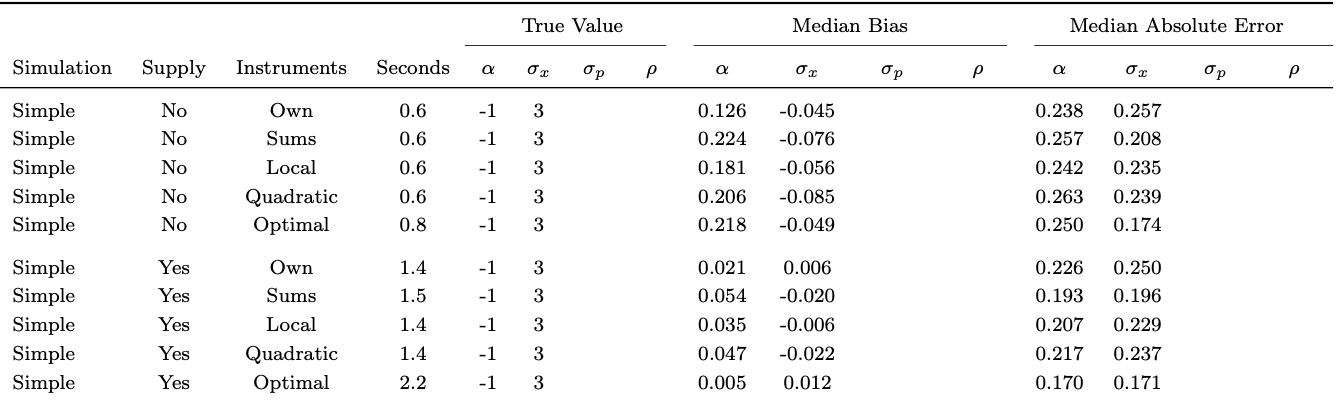
\includegraphics[width=0.75\textwidth]{resources/supply_table}
\end{center}
\end{frame}



\begin{frame}{What about Misspecification? (Conlon Gortmaker RJE 2020)}
\begin{center}
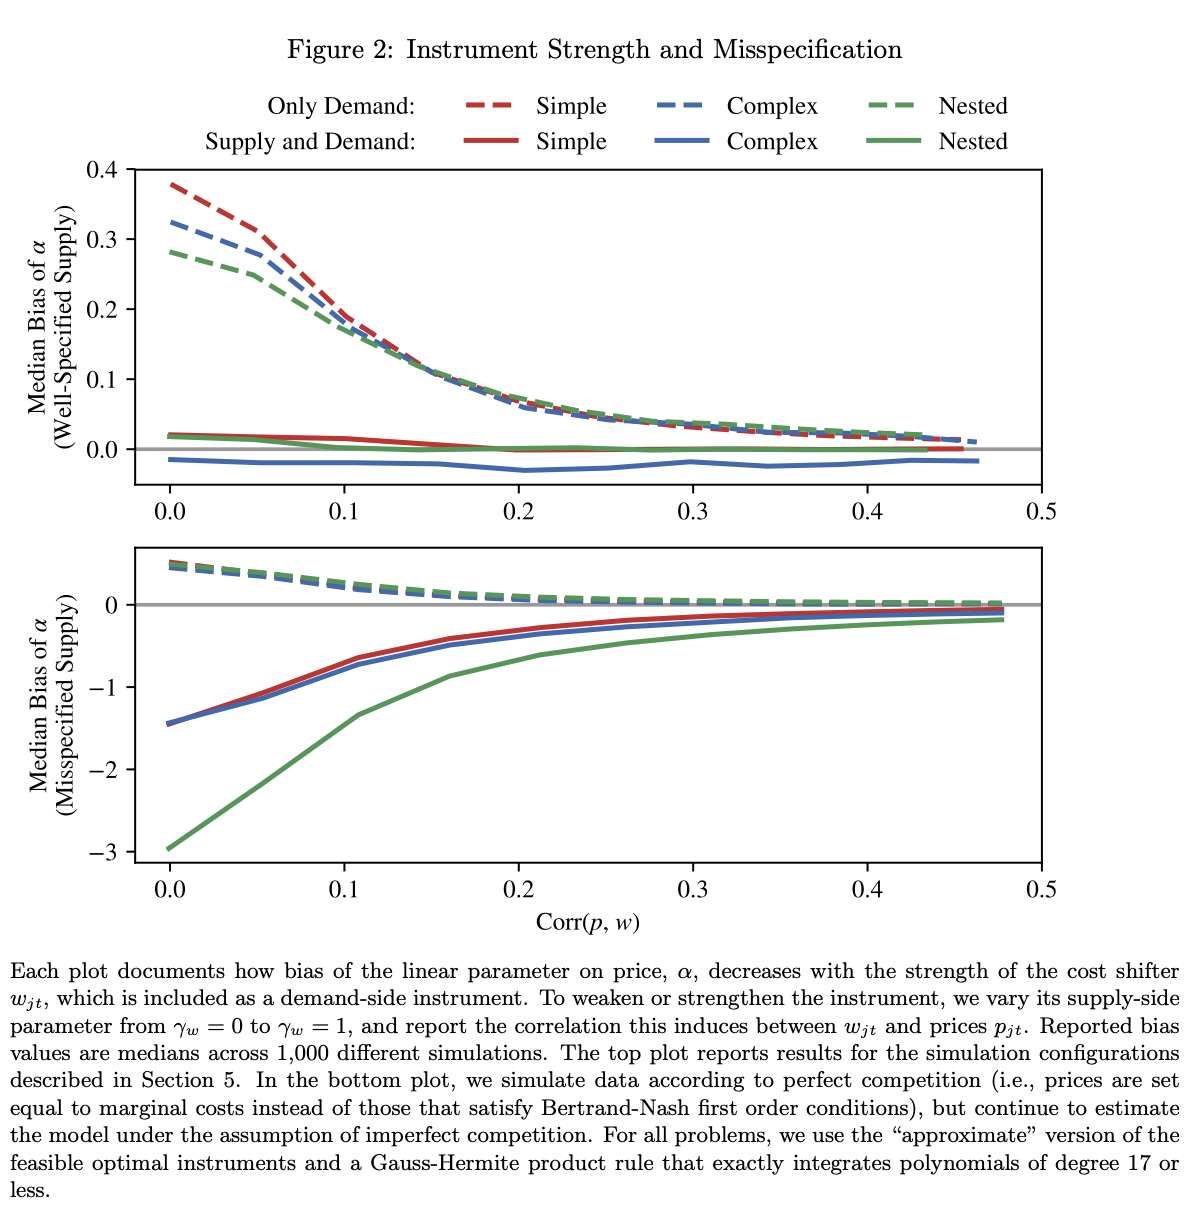
\includegraphics[height=0.9\textheight]{resources/supply_figure}
\end{center}
\end{frame}

%
%
%
%
%\begin{frame}{Supply Side as Instruments }
%\begin{itemize}
%\item Instruments for demand depend on \alert{exclusion restrictions}
%\item Where do instruments come from? Something omitted that appears in another equation.
%\end{itemize}
%\begin{eqnarray*}
%p_{jt}  &=& c_{jt}(w_{jt},x_{jt}) +  \frac{s_{jt}(\mathbf{p_t})}{\left|\frac{\partial s_{jt}(\mathbf{p_t})}{\partial p_{jt}}\right|}  +\sum_{k \in \mathcal{J}_f} (p_k - c_k) \frac{\frac{ \partial s_{kt}}{\partial p_{jt}}(\mathbf{p_t})}{\left|\frac{\partial s_{jt}(\mathbf{p_t})}{\partial p_{jt}}\right|}  
%\end{eqnarray*}
%\begin{enumerate}
%\item Exogenous regressors $x_{jt}$.
%\item Cost shifters: $w_{jt}$ (hard to find in practice), Hausman instruments.
%\item Markup shifters:  $ \frac{s_{jt}(\mathbf{p_t})}{\frac{\partial s_{jt}(\mathbf{p_t})}{\partial p_{jt}}}$ \\(function of $(p_j,x_j,\xi_j, p_{-j},x_{-j},\xi_{-j})$).
%\end{enumerate}
%\end{frame}
%

%
%\begin{frame}{Differentiation Instruments: Gandhi Houde (2016)}
%\begin{center}
%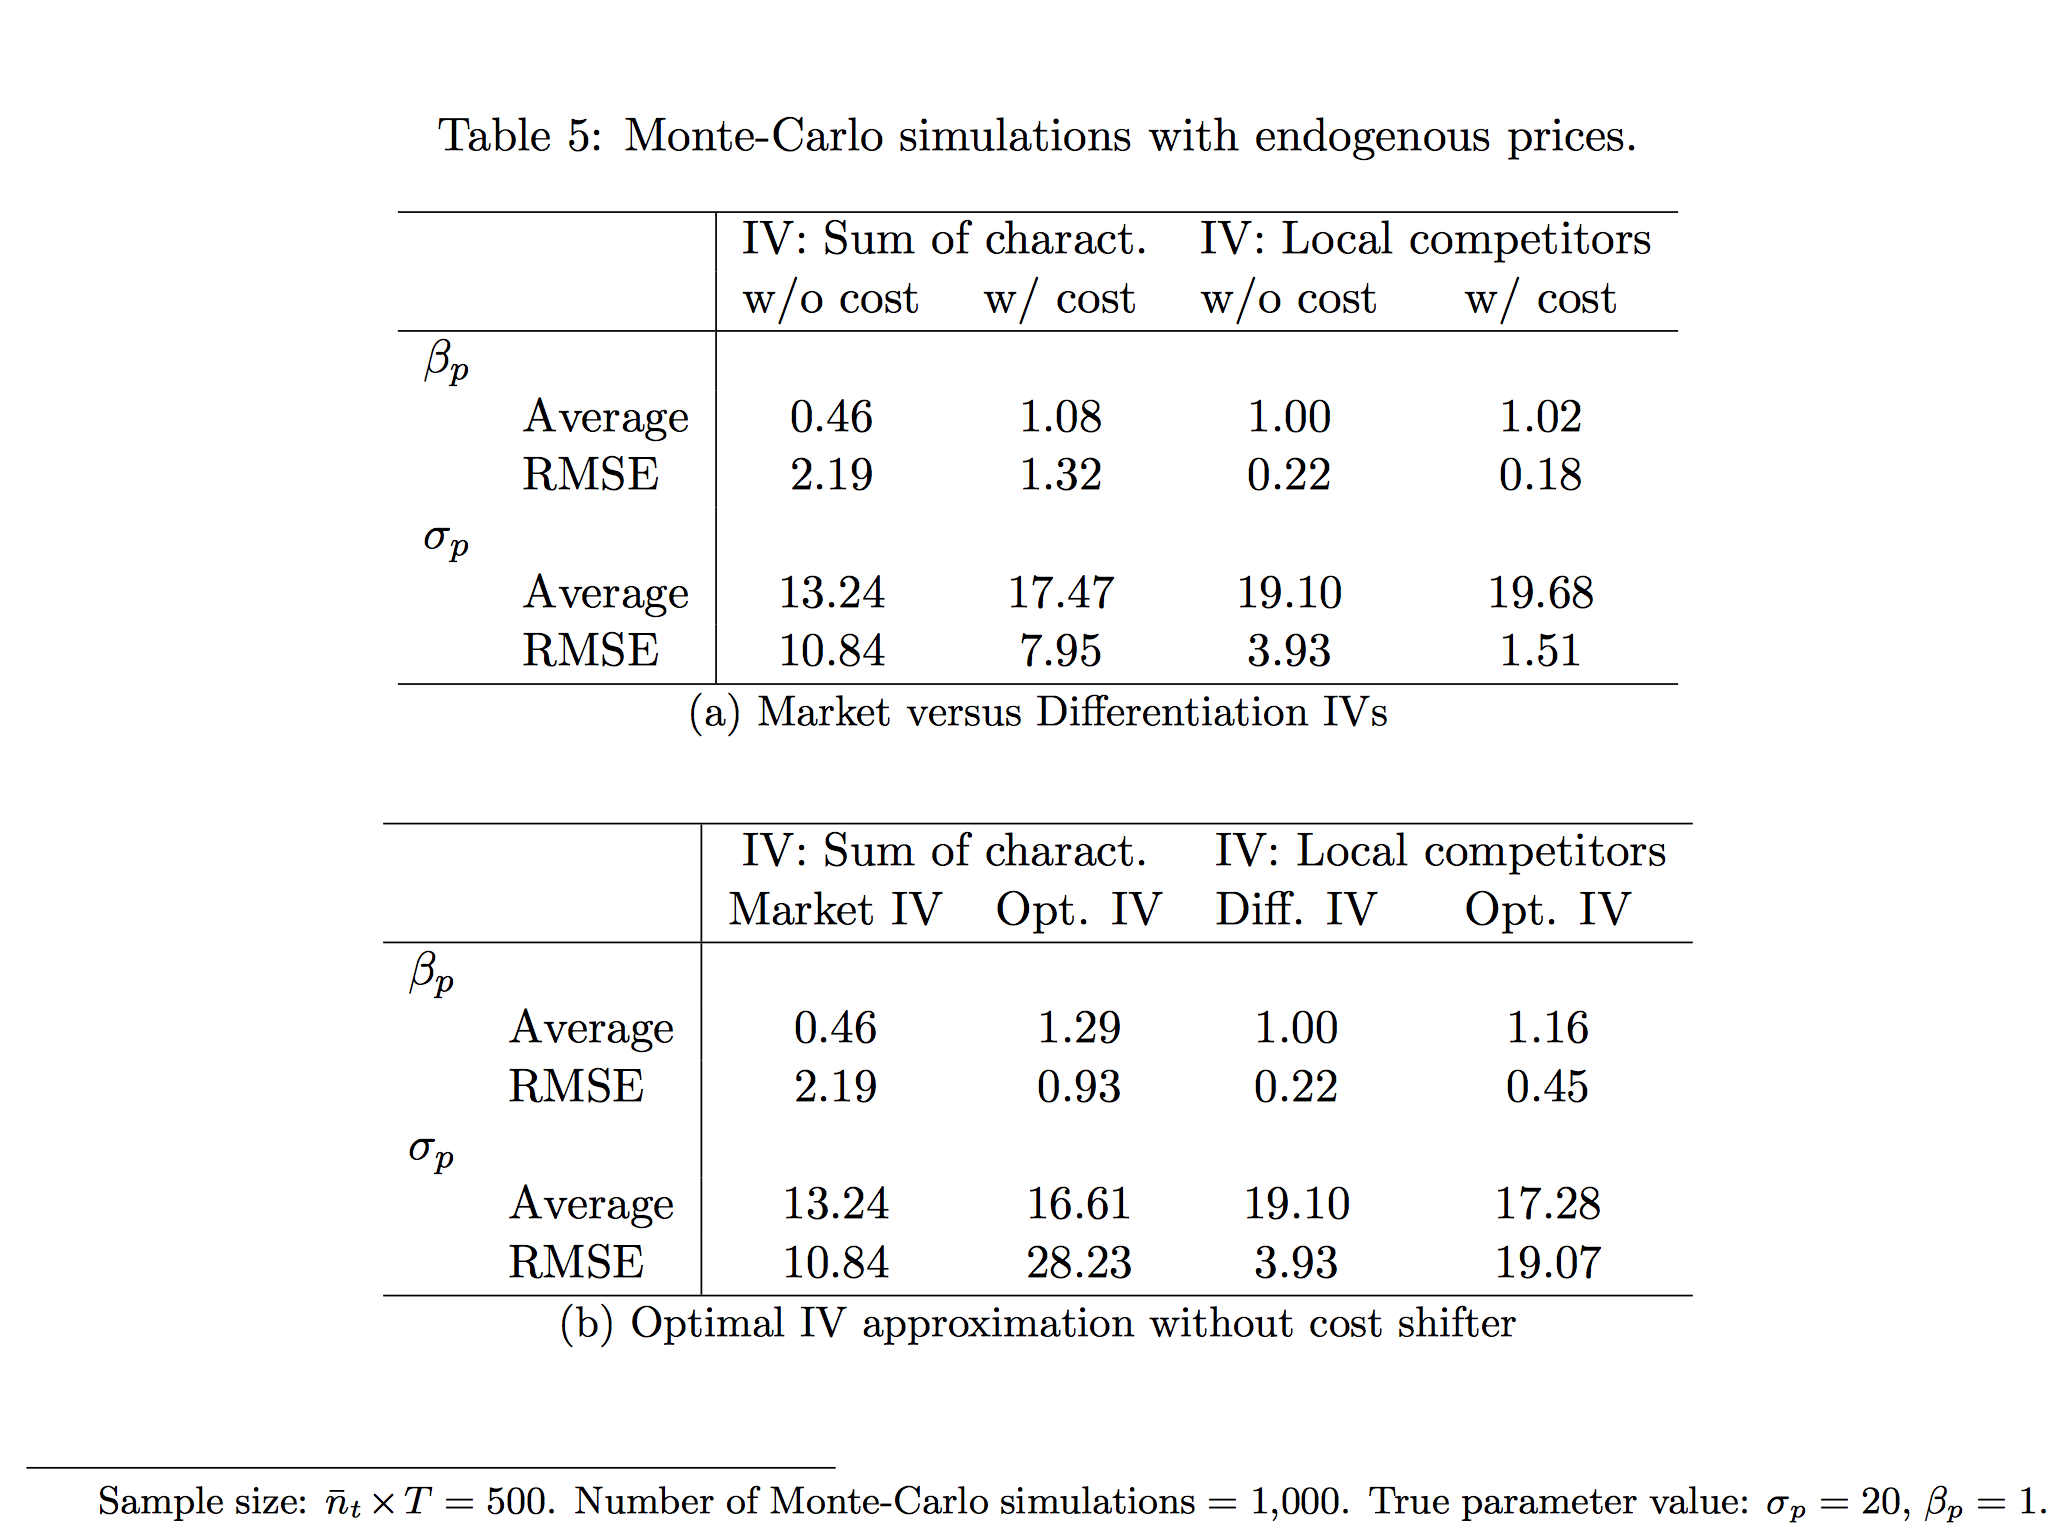
\includegraphics[width=3.8in]{resources/d_iv2.png}
%\end{center}
%\end{frame}
%



%
%\begin{frame} \frametitle{Extensions: Supply Moments}
%\begin{itemize}
%\item We can also impose the Bertrand FOC as a set of additional moments.
%\item First parametrize marginal cost
%\begin{eqnarray*}
%\ln mc_{jt} = \gamma_1 x_{jt} + \gamma_2 w_{jt} + \omega_{jt}
%\end{eqnarray*}
%\item helpful to constrain MC to be positive always.
%\item Note that for any vector of prices $p$ and demand parameters $\theta$ we can recover a unique vector of marginal costs (by solving the system of linear equations).
%\item Imposing these restrictions is helpful in constraining markups (so that implied MC are always positive, etc.).
%\item Misspecified functional forms for costs can cause problems!
%\end{itemize}
%\end{frame}





\end{document}